%---------------------------------------------------------------------------
% System Decomposition.
%
%---------------------------------------------------------------------------
\section{Decomposition}
\label{sec:arch_decomposition}

The high level system architecture is depicted in figure~\ref{fig:arch_overall}. 

\begin{figure}[ht]
\centering
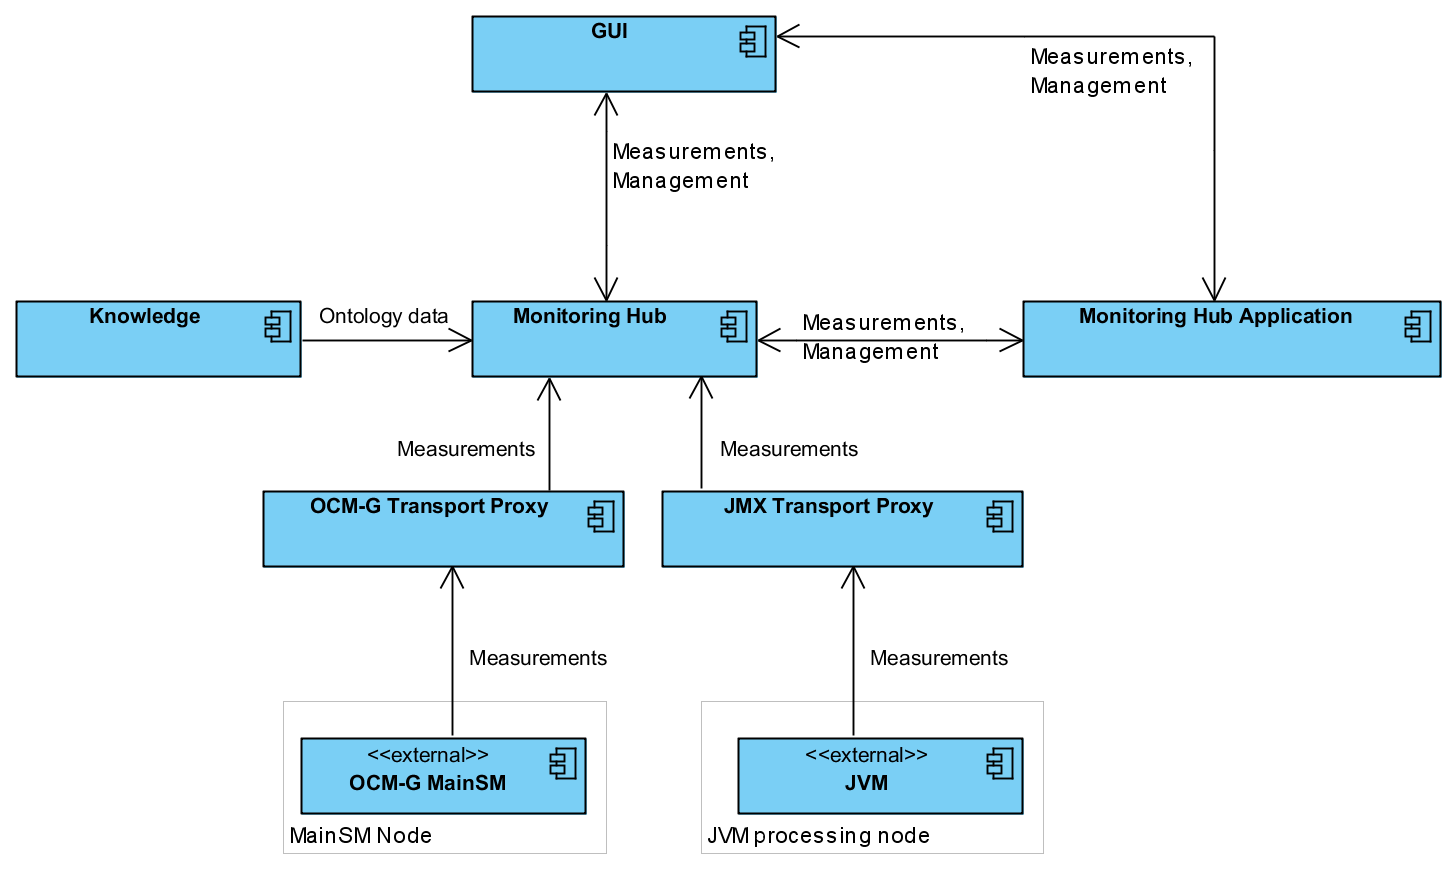
\includegraphics[width=1\textwidth]{arch_flows}
\caption{Overall system architecture}
\label{fig:arch_overall}
\end{figure}

During the design stage, several high level components have been introduced. All distinguished components, with relationships between them can be found in Figure~\ref{fig:decomposition_overall}. Each of those components should be interpreted as independent one, which means that it is either standalone application or library, with API containing one or more interfaces. This API is then shared between provider, which is a component that realizes given interface and consumer - module that uses those functionalities to realize its own aims. Following subsection tries to list those components and describe them roughly.

\begin{figure}[ht]
\centering
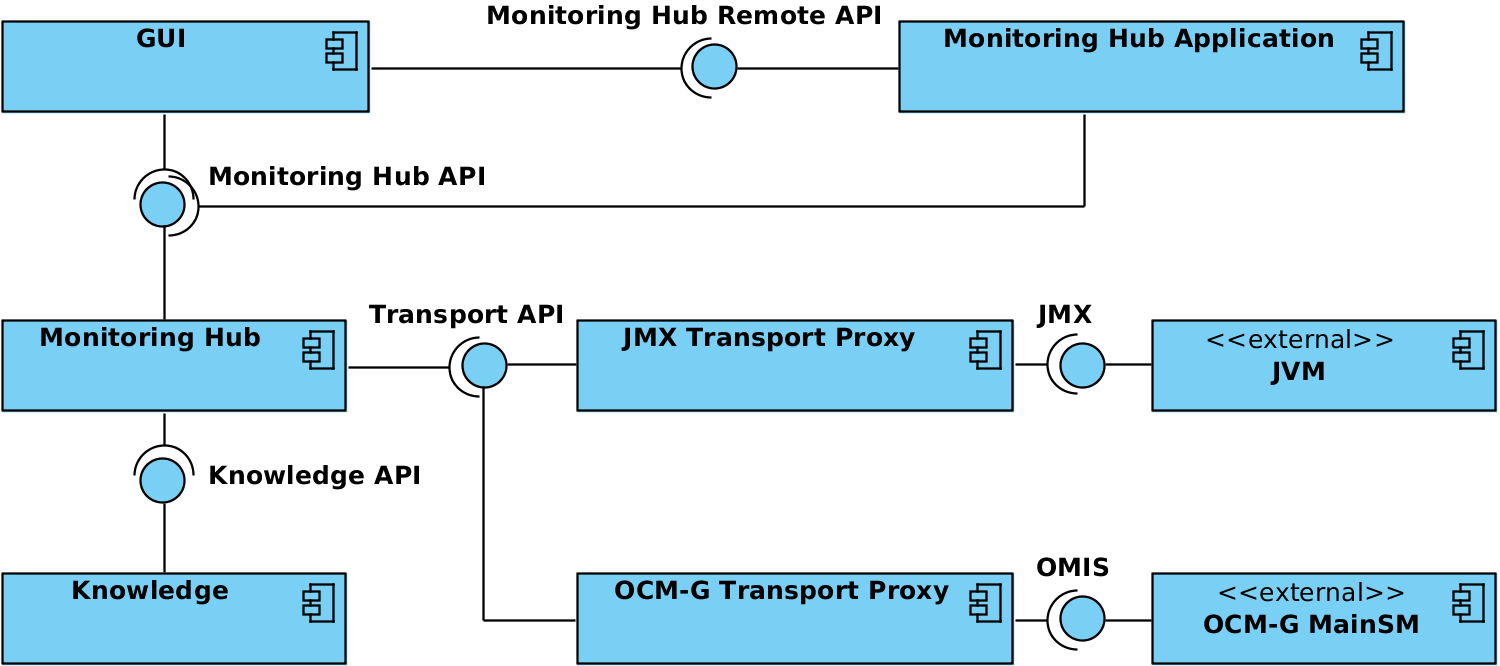
\includegraphics[width=1\textwidth]{arch_overall}
\caption{Overall system decomposition}
\label{fig:decomposition_overall}
\end{figure}

\subsection{Components overview}

As can be seen in Figure~\ref{fig:arch_overall}, system has been decomposed into 8 high-level components. Those are:

\begin{itemize}

\item {\bf GUI}~~~~~~~~~~~~~~~~~~~~~~~~~~~~~~~~~~~~~~~~~~~~~~~~~~~~~~~~\linebreak
Graphic User Interface is standalone, desktop application, used directly by the user. It provides facilities that allow management of the whole system. It does not perform any measurements or analysis. It only gives control over other components (direct or indirect) and visualizes results of measurements.
GUI application contains embedded Monitoring Hub, which allows the system to operate also in smallest scale - single measuring process with one or more measured processes attached directly. Additionally it connects to Monitoring Hub Application which allows using remote Monitoring Hub.

\item {\bf Monitoring Hub}~~~~~~~~~~~~~~~~~~~~~~~~~~~~~~~~~~~~~~~~~~~~~~~~~~~~~~~~\linebreak
Monitoring hub is most crucial component. Contains all logic needed for resources and measurements management. It uses Knowledge and Transport Proxies (one or more implementation) components, to fulfill its duties. Only JMX and OCM-G transport proxies will be provided at this stage of development, but proposed architecture allows easy addition of new proxies.
Monitoring Hub does not work as standalone application. Instead, it is in the form of library (Java JAR) that other components will use. Additionally, Monitoring Hub component is used by GUI (in embedded mode) and Monitoring Hub Application.

\item {\bf Monitoring Hub Application}~~~~~~~~~~~~~~~~~~~~~~~~~~~~~~~~~~~~~~~~~~~~~~~~~~~~~~~~\linebreak
Monitoring Hub Application will be standalone, command line application (or daemon if possible) that exposes services of Monitoring Hub to other components with remote access through the network (either LAN or WAN). It can accept remote connections from GUI components.
Its main responsibility is to allow the system to work in distributed manner. Having a process that is separate, and independent from GUI application, which continuously measures work of long-lasting jobs is crucial to allow the system to scale up.


\item {\bf Knowledge}~~~~~~~~~~~~~~~~~~~~~~~~~~~~~~~~~~~~~~~~~~~~~~~~~~~~~~~~\linebreak
Knowledge component realizes semantic approach of application. It provides ontology functionalities to Monitoring Hub. It is responsible for initializing ontology database and response to all queries issued by Monitoring Hub regarding relationships between resource types, resources or capabilities. This component is in the form of a library that is a dependency for Monitoring Hub, and must be included in both GUI and Monitoring Hub Application distributions.

\item {\bf JMX Transport Proxy}~~~~~~~~~~~~~~~~~~~~~~~~~~~~~~~~~~~~~~~~~~~~~~~~~~~~~~~~\linebreak
Transport proxy component, which can communicate with JVM processes using JMX protocol. Its main responsibilities include: establishing a connection with JVM, mapping between generic, knowledge-based resources or capability value requests into Java components or JMX queries.

\item {\bf OCM-G Transport Proxy}~~~~~~~~~~~~~~~~~~~~~~~~~~~~~~~~~~~~~~~~~~~~~~~~~~~~~~~~\linebreak
Transport proxy component that communicates with OCM-G MainSM monitor. Its responsibilities are similar to those of JMX Transport Proxy - establish and maintain connection to MainSM, translate queries given in ontology terms to OMIS requests.

\end{itemize}

\subsection{Interfaces overview}

To decouple all proposed components, system will be using following interfaces:

\begin{itemize}

\item {\bf Monitoring Hub API}~~~~~~~~~~~~~~~~~~~~~~~~~~~~~~~~~~~~~~~~~~~~~~~~~~~~~~~~\linebreak
Interface for core system's logic. Describes methods that allow managing of every aspect of system - measurements, visualizations and resources management. It is realized by Monitoring Hub component and used by GUI. 

\item {\bf Monitoring Hub Remote API}~~~~~~~~~~~~~~~~~~~~~~~~~~~~~~~~~~~~~~~~~~~~~~~~~~~~~~~~\linebreak
This interface is a derivative of Monitoring Hub API. It contains same set of functionalities, with addition of operations specific to remote access. This includes: registration of remote listener, remote interface wrapper for Monitoring Hub allowing passing remote exceptions.

\item {\bf Transport API}~~~~~~~~~~~~~~~~~~~~~~~~~~~~~~~~~~~~~~~~~~~~~~~~~~~~~~~~\linebreak
Transport API is common interface for communication with data access services. Currently it is implemented by JMX and OCM-G Transport Proxy component. To add support of other data sources in future - this interface will have to be implemented.

\item {\bf Knowledge API} ~~~~~~~~~~~~~~~~~~~~~~~~~~~~~~~~~~~~~~~~~~~~~~~~~~~~~~~~\linebreak
Interface describing operations related to ontology maintenance and usage. This interface is realized by Knowledge component and used by Monitoring Hub. 

\end{itemize}

\subsection{Most important data flows}

\begin{figure}[ht]
\centering
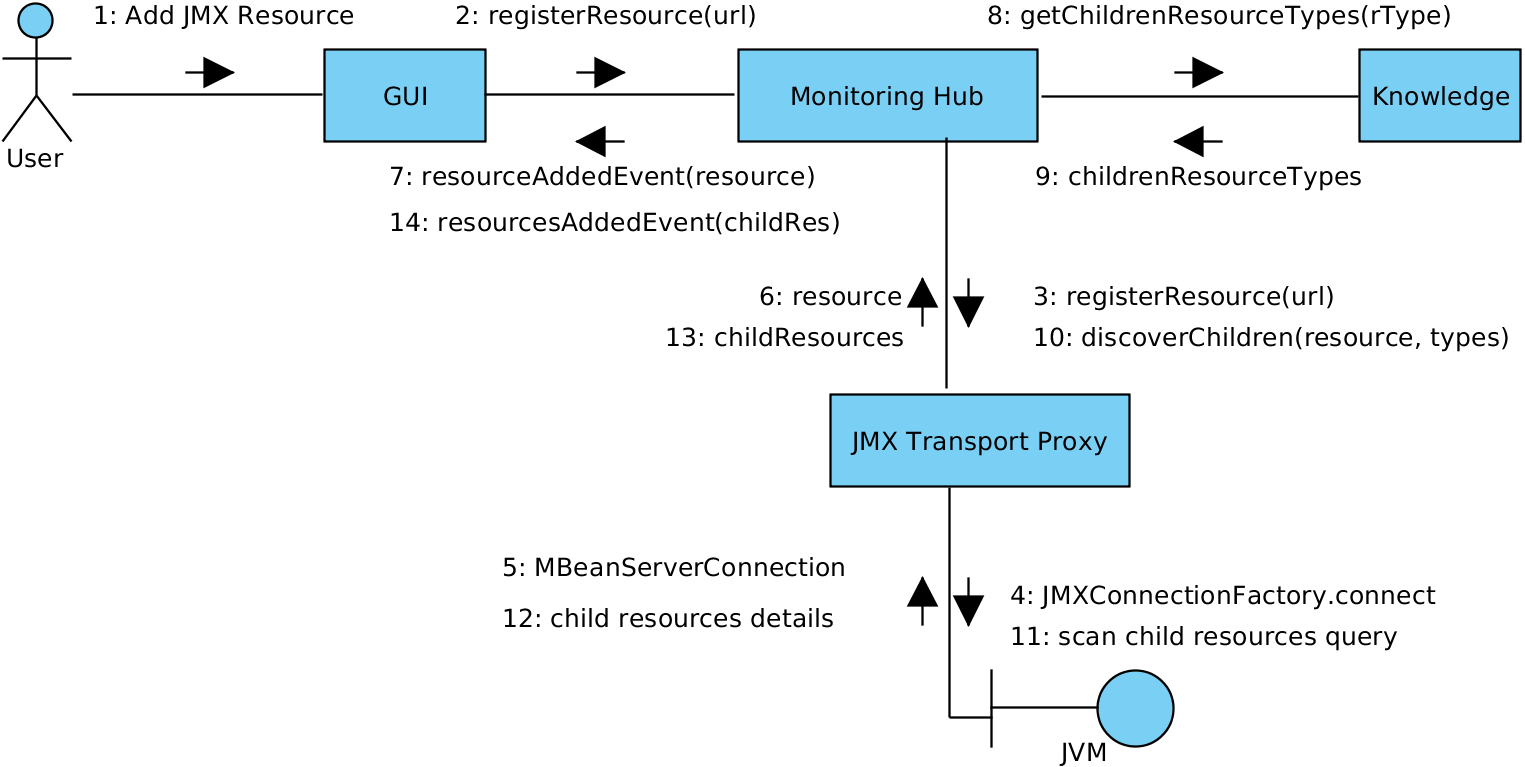
\includegraphics[width=0.9\textwidth]{comm_add_resource}
\caption{Communication diagram - adding of new resource}
\label{fig:comm_add_resource}
\end{figure}

Figure~\ref{fig:comm_add_resource} contains communication diagram covering addition of new resource action. This action is initialized by User actor. User starts flow by performing action (like button click or wizard - not covered here) on GUI component. In response to this event, GUI sends request to Monitoring Hub, asking to register new resource, using parameters provided by the user. In subsequent step, Monitoring Hub first lookups for the one that can communicate with resource specified by user in its dictionary of all registered transport proxies. After finding valid transport proxy, it passes the registration request to it. In this case, JMX Transport Proxy tries to initialize connection to JVM using URL provided by user in first step. After successful connection, JVM creates and initializes Resource object. This process includes gathering basic attributes describing object as well as setting all meta data that proxy will need to operate with given resource in future. After finishing this step, fully initialized resource is being returned to Monitoring Hub. Knowing that transport proxy has been properly attached to newly registered resource, Monitoring Hub notifies about new resource all listeners - in this case GUI component. After issuing this notification, it will try to discover all children of this resource. To achieve that, first it must obtain URLs of child types, so it sends a request to the Knowledge component. Having types of child resources, Monitoring Hub requests transport proxy to discover children of already registered resource and of given types. Again, in this case JMX transport proxy will translate discovery request into JMX queries, to discover child resources. Discovered children are then returned to Monitoring Hub as resource objects. All those object are registered by Hub and notification is being issued to listeners.

\begin{figure}[ht]
\centering
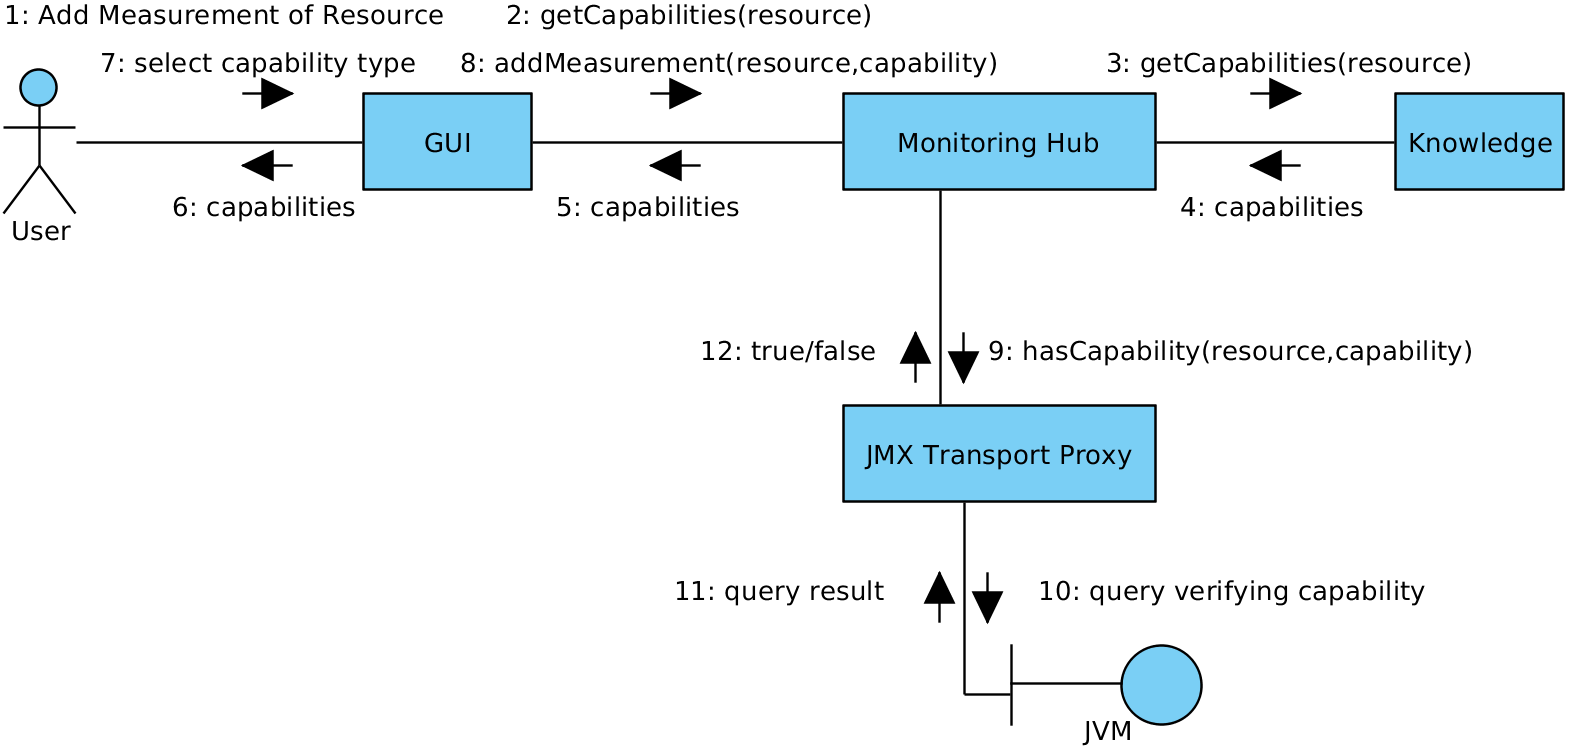
\includegraphics[width=0.9\textwidth]{comm_add_measurement}
\caption{Communication diagram - adding of new measurement}
\label{fig:comm_add_measurement}
\end{figure}

Addition of new measurement is a bit simpler than registration of new resources. All messages exchange needed to achieve it can be found in Figure~\ref{fig:comm_add_measurement}. In this case, same as above, action is initialized by a user. He or she chooses resource to add measurement of, and clicks appropriate button. In reaction to this event, GUI requests Monitoring Hub to get all possible capabilities that can be measured for resource type of resource selected by the user. Monitoring Hub passes this request to Knowledge component. Then, a result goes back GUI, which can render appropriate user interface item that will allow user to select which capability to measure. After selecting capability by user, GUI issues request to add new measurement to Monitoring Hub. The request contains both resource identifier and ontology URL of capability. Monitoring Hub verifies then, whether selected capability can be measured with the selected resource. Such a validation is needed, because in certain circumstances it might be impossible. To check this, Monitoring Hub sends verification request to transport proxy (JMX Transport Proxy in example from Figure~\ref{fig:comm_add_measurement}). After successful verification, Monitoring Hub initializes scheduler that will poll for capability values - measurement is successfully created and started.

\begin{figure}[ht]
\centering
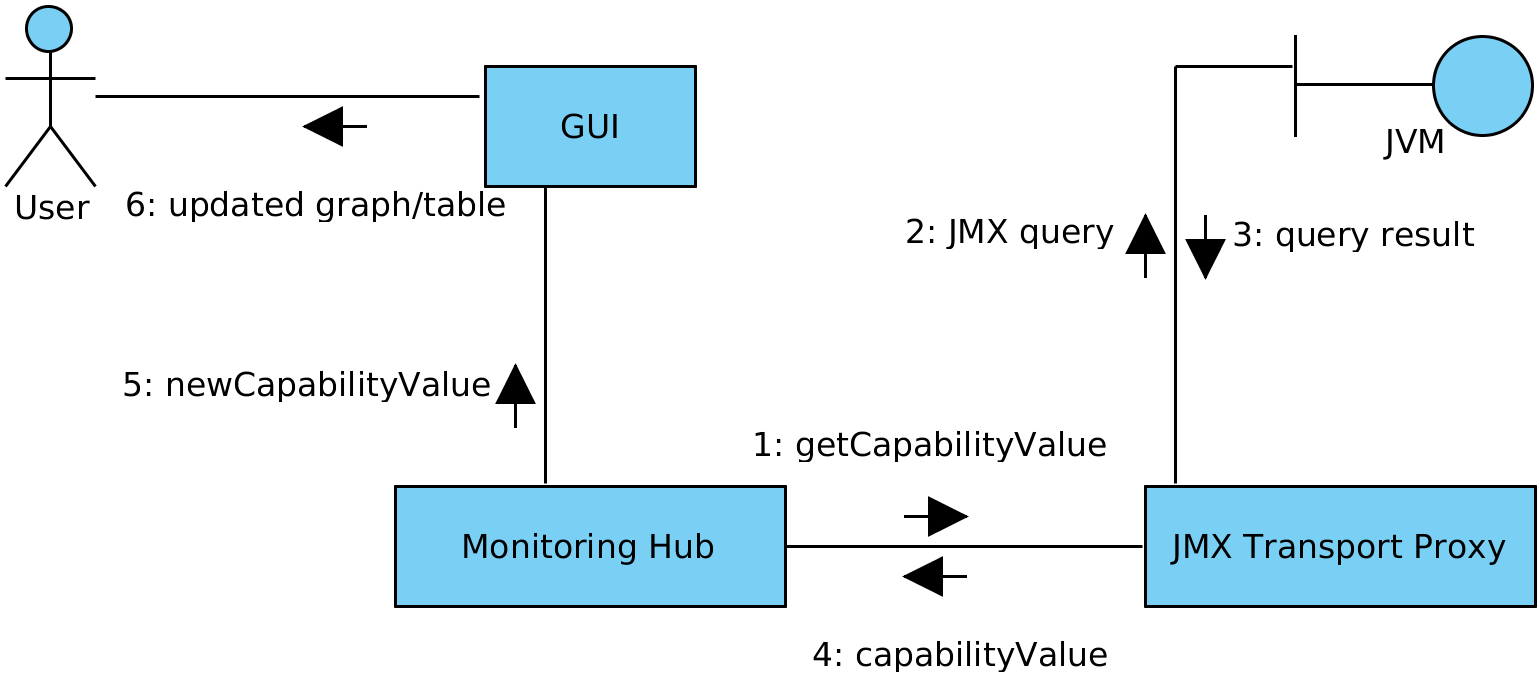
\includegraphics[width=0.7\textwidth]{comm_new_cap_value}
\caption{Communication diagram - new capability value}
\label{fig:comm_new_cap_value}
\end{figure}

Publishing new capability value is definitely most frequently used data flow in whole system. Figure~\ref{fig:comm_new_cap_value} depicts this process. In contrast to previous communication diagrams, in this case the Monitoring Hub component is initiator of this operation. Logic of this component manages scheduled jobs responsible for polling of new capability value, and then pushing to listeners - previously registered GUI components. In first step, Monitoring Hub calls appropriate (the one associated with resource in question) transport proxy, which is JMX Transport Proxy in this case. JMX Transport Proxy maps generic getCapabilityValue request into specific JMX query, sends the query to monitored JVM and returns result to Hub. Monitoring Hub uses this result to issue notification dispatched through all registered listeners. GUI component, receives event and updates visualization graph, which is being watched by a user.

\subsection{Communication protocol}
\label{subsec:arch_comm_protocol}

Communication protocol between components must allow both types of interactions: local and remote. By local interaction I mean the one, where all components constitute single process and share same memory space. Remote system must use remote interaction, when one or more components works as a separate process to other which enforces usage of network stack for messages exchange. To make it possible, all communications will be performed using predefined, plain interfaces, which aren't aware of underlying communication type. Such an approach decouples communication schema from networking protocol being employed.

As a general rule for all message exchanges between components, Transfer Object (also known as Value Object) design pattern will be used\cite{0131422464}. This allows decoupling content of message of any complexity from serialization mechanisms used. Following tables list all transfer objects used in system. Additionally reader may find short description of each object rationale behind each member. 

% Add vertical spacing
\renewcommand*\arraystretch{1.2}

\begin{table}[ht] % ======================== CapabilityValue =====================================
\begin{tabular}{| m{1,5cm} | m{2,5cm} | m{8,5cm} |}
\hline 
\cellcolor[gray]{0.9} Field Type & \cellcolor[gray]{0.9} Field Name & \cellcolor[gray]{0.9} Details \\
\hline 
Number & numberValue & Numeric value of capability (optional, must be set if ValueType is number) \\
Number[] & arrayValue & Vector value of capability (optional, must be set if ValueType is vector) \\
ValueType & valueType & Type of capability value - either numeric or vector\\
Date & gatherTimestamp & Timestamp in UTF, when capability value have been gathered \\
String & metricsId & Id of measurement to which this capability value belongs \\
\hline 
\end{tabular}
\caption{List of members of CapabilityValue Transfer Object}
\label{tab:TO_CapValue}
\end{table} % ======================== CapabilityValue =====================================

Table~\ref{tab:TO_CapValue} contains list of members of CapabilityValue transfer object. This object is used to notify listeners (GUI) about new capability values, and acts mostly as container for value, with additional metadata. Most significant additional property that each CapabilityValue has is gatherTimestamp which points to exact moment of time, when this capability value has been gathered. Using this property, system can use CapabilityValue transfer objects, without worrying about implication of processing time on measurements presentation.

Members of MeasurementDefinition message format can be found in Table~\ref{tab:TO_MeasurementDef}. This object is used by GUI component to define measurement that should be created during createMeasurement request.

\begin{table}[ht] % ======================== MeasurementDefinition =====================================
\begin{tabular}{| m{1,5cm} | m{2,5cm} | m{8,5cm} |}
\hline 
\cellcolor[gray]{0.9} Field Type & \cellcolor[gray]{0.9} Field Name & \cellcolor[gray]{0.9} Details \\
\hline 
String & resourceUri & Uri of resource that is covered by this measurement \\
String & capabilityUri & Uri of capability that is covered by this measurement \\
long & updateInterval & Interval in milliseconds defining how frequently value of measurement will be polled \\
String & id & Identifier of this measurement \\ 
\hline 
\end{tabular}
\caption{List of members of MeasurementDefinition Transfer Object}
\label{tab:TO_MeasurementDef}
\end{table} % ======================== MeasurementDefinition =====================================

Following tables:~\ref{tab:TO_Resource} and \ref{tab:TO_ResourceEvent} contains transfer objects needed for resource management. Resource transfer object contains complete description of resource managed by system, additionally MonitoringHub uses ResourceEvent to notify all listeners (GUI mostly) about resource's life cycle events. 

\begin{table}[ht] % ======================== Resource =====================================
\begin{tabular}{| m{1,5cm} | m{2,5cm} | m{8,5cm} | }
\hline 
\cellcolor[gray]{0.9} Field Type & \cellcolor[gray]{0.9} Field Name & \cellcolor[gray]{0.9} Details \\
\hline
String & typeUri & URI of resource\rq{}s type according to currently used ontology \\
String & uri & URI of resource in current resources tree hierarchy \\
Map & properties & Static properties of resource (e.g. OS version) \\
\hline 
\end{tabular}
\caption{List of members of Resource Transfer Object}
\label{tab:TO_Resource}
\end{table} % ======================== Resource =====================================

\begin{table}[ht] % ======================== ResourceEvent =====================================
\begin{tabular}{| m{1,5cm} | m{2,5cm} | m{8,5cm} | }
\hline 
\cellcolor[gray]{0.9} Field Type & \cellcolor[gray]{0.9} Field Name & \cellcolor[gray]{0.9} Details \\
\hline
Type & eventType & Enumeration that defines whether resources in this event have been added or removed \\
List & resources & Collections of resources covered by this event \\
\hline 
\end{tabular}
\caption{List of members of ResourceEvent Transfer Object}
\label{tab:TO_ResourceEvent}
\end{table} % ======================== ResourceEvent =====================================
% Remove vertical spacing
\renewcommand*\arraystretch{1}

